% ============================================================================
%  SLIDE THUYẾT TRÌNH — CS221 · Transformer cho đọc hiểu tiếng Việt
%  Dùng CHUNG số liệu với báo cáo: ../report/generated/numbers.tex (sinh từ results/)
%  Biên dịch:  cd slides && latexmk -xelatex main.tex
%
%  GIAO DIỆN: hệ thiết kế "Organic" của web demo (demo/console/theme.py) — cùng
%  token màu, cùng kiểu chữ, để slide và demo trông như một sản phẩm. Báo cáo
%  (report/) giữ nguyên bảng màu xanh/cam của nó.
%
%  CẦN CÀI PHÔNG (một lần, mỗi máy):
%    Be Vietnam Pro  https://fonts.google.com/specimen/Be+Vietnam+Pro
%    Source Code Pro https://fonts.google.com/specimen/Source+Code+Pro
%  Hai phông này có đủ bộ ký tự tiếng Việt; đây cũng là phông của web demo.
% ============================================================================
\documentclass[aspectratio=169,11pt]{beamer}
\usetheme[progressbar=frametitle,numbering=fraction,block=fill]{metropolis}
\usepackage{fontspec}
\setsansfont{Be Vietnam Pro}
\newfontfamily\headfont{Be Vietnam Pro ExtraBold}
\setmonofont{Source Code Pro}[Scale=0.90]
\usepackage{booktabs,tabularx,array,graphicx,xcolor,tikz,colortbl}
\usetikzlibrary{arrows.meta,positioning,calc}

% ── token hệ thiết kế Organic (demo/console/theme.py) ───────────────────────
\definecolor{orgbg}{HTML}{F5EAD8}        % --color-bg
\definecolor{orgsurface}{HTML}{EBDDC5}   % --color-surface
\definecolor{orgcard}{HTML}{F9F4ED}      % --color-neutral-100  (.vm-card)
\definecolor{orgaccent}{HTML}{C67139}    % --color-accent
\definecolor{orgaccent2}{HTML}{7A8A5E}   % --color-accent-2
\definecolor{orgacc100}{HTML}{FFF2EB}    % --color-accent-100
\definecolor{orgacc600}{HTML}{B2622D}
\definecolor{orgacc700}{HTML}{8C491A}
\definecolor{orgacc800}{HTML}{643312}
\definecolor{orgacc2600}{HTML}{728157}
\definecolor{orgacc2700}{HTML}{56633F}
\definecolor{orgn200}{HTML}{EEE7DB}
\definecolor{orgn300}{HTML}{DCD3C4}
\definecolor{orgn500}{HTML}{A19786}
\definecolor{orgn700}{HTML}{645C50}

% ── tên ngữ nghĩa dùng trong body.tex (giữ nguyên, chỉ đổi giá trị) ─────────
\definecolor{orgink}{HTML}{201E1D}       % --color-text
\colorlet{ink}{orgink}
\colorlet{muted}{orgn700}
\colorlet{phobert}{orgaccent}            % PhoBERT  → terracotta (accent)
\colorlet{xlmr}{orgaccent2}              % XLM-R    → ô liu (accent-2)
\colorlet{tfidf}{orgn700}                % TF-IDF → trung tính đậm (5,53:1 trên nền kem)
\colorlet{badred}{orgacc700}
\colorlet{okgreen}{orgacc2700}
\colorlet{warnorange}{orgacc600}
\colorlet{uitblue}{orgaccent}
\colorlet{soft}{orgcard}

% ── ánh xạ token sang Beamer ────────────────────────────────────────────────
\setbeamercolor{background canvas}{bg=orgbg}
\setbeamercolor{normal text}{fg=orgink,bg=orgbg}
\setbeamercolor{frametitle}{bg=orgsurface,fg=orgink}
\setbeamercolor{progress bar}{fg=orgaccent,bg=orgn300}
\setbeamercolor{progress bar in head/foot}{fg=orgaccent,bg=orgn300}
\setbeamercolor{alerted text}{fg=orgacc600}
\setbeamercolor{example text}{fg=orgacc2600}
\setbeamercolor{block title}{bg=orgacc100,fg=orgacc800}   % .vm-card + .vm-tag-accent
\setbeamercolor{block body}{bg=orgcard,fg=orgink}
\setbeamercolor{title separator}{fg=orgaccent}
\setbeamercolor{palette primary}{bg=orgsurface,fg=orgink}
\setbeamercolor{section title}{fg=orgink}
\setbeamercolor{footline}{fg=orgn700}
\setbeamerfont{frametitle}{family=\headfont,size=\large}
\setbeamerfont{title}{family=\headfont,size=\Large}
\setbeamerfont{section title}{family=\headfont,size=\LARGE}
\setbeamerfont{block title}{series=\bfseries}
% .vm-card: bo góc lớn, không viền, nền sáng hơn nền trang
\setbeamertemplate{blocks}[rounded][shadow=false]

\newcommand{\code}[1]{\texttt{#1}}
% SINH TỰ ĐỘNG bởi scripts/make_report_numbers.py — KHÔNG SỬA TAY
\providecommand{\missing}{\textcolor{badred}{\textbf{??}}}
\newcommand{\NTrain}{28.454}
\newcommand{\NTrainCtx}{4.101}
\newcommand{\NTrainImp}{9.216}
\newcommand{\PctTrainImp}{32{,}39}
\newcommand{\NTrainAns}{19.238}
\newcommand{\NVal}{3.814}
\newcommand{\NValCtx}{557}
\newcommand{\NValImp}{1.161}
\newcommand{\PctValImp}{30{,}44}
\newcommand{\NValAns}{2.653}
\newcommand{\NFit}{27.049}
\newcommand{\NFitCtx}{3.896}
\newcommand{\NFitImp}{8.773}
\newcommand{\PctFitImp}{32{,}43}
\newcommand{\NFitAns}{18.276}
\newcommand{\NDev}{1.405}
\newcommand{\NDevCtx}{205}
\newcommand{\NDevImp}{443}
\newcommand{\PctDevImp}{31{,}53}
\newcommand{\NDevAns}{962}
\newcommand{\SegN}{2.653}
\newcommand{\SegAligned}{2.620}
\newcommand{\SegMis}{33}
\newcommand{\SegStartCut}{13}
\newcommand{\SegEndCut}{20}
\newcommand{\SegCtx}{557}
\newcommand{\SegMisPct}{1{,}24}
\newcommand{\SegOracle}{99{,}25}
\newcommand{\SegOracleMis}{39{,}39}
\newcommand{\SegAlignedPct}{98{,}76}
\newcommand{\SegCeilingLoss}{0{,}75}
\newcommand{\SegCtxCoverage}{100{,}00}
\newcommand{\MisPeriod}{13}
\newcommand{\MisMerge}{12}
\newcommand{\MisCompound}{3}
\newcommand{\MisAnnot}{5}
\newcommand{\AuditN}{250}
\newcommand{\AuditAns}{120}
\newcommand{\AuditAnsInCtx}{15}
\newcommand{\AuditOffsetOK}{6}
\newcommand{\AuditValid}{145}
\newcommand{\AuditCtx}{5}
\newcommand{\AuditFlat}{120}
\newcommand{\AuditCombined}{370}
\newcommand{\AuditTrainOverlap}{0}
\newcommand{\AuditEOneValid}{14}
\newcommand{\AuditEOneAns}{41}
\newcommand{\AuditEOneAnsInCtx}{5}
\newcommand{\AuditEOneDistinctQ}{21}
\newcommand{\AuditETwoValid}{17}
\newcommand{\AuditETwoAns}{35}
\newcommand{\AuditETwoAnsInCtx}{2}
\newcommand{\AuditETwoDistinctQ}{28}
\newcommand{\AuditEThreeValid}{50}
\newcommand{\AuditEThreeAns}{0}
\newcommand{\AuditEThreeAnsInCtx}{0}
\newcommand{\AuditEThreeDistinctQ}{14}
\newcommand{\AuditEFourValid}{18}
\newcommand{\AuditEFourAns}{37}
\newcommand{\AuditEFourAnsInCtx}{5}
\newcommand{\AuditEFourDistinctQ}{13}
\newcommand{\AuditEFiveValid}{46}
\newcommand{\AuditEFiveAns}{7}
\newcommand{\AuditEFiveAnsInCtx}{3}
\newcommand{\AuditEFiveDistinctQ}{8}
\newcommand{\AbstainEM}{30{,}44}
\newcommand{\AbstainFone}{30{,}44}
\newcommand{\AbstainAnsEM}{0{,}00}
\newcommand{\AbstainAnsFone}{0{,}00}
\newcommand{\AbstainImpEM}{100{,}00}
\newcommand{\AbstainLat}{0{,}00}
\newcommand{\AbstainStressEM}{52{,}00}
\newcommand{\AbstainAbsRate}{100{,}00}
\newcommand{\AbstainAbsPrec}{30{,}44}
\newcommand{\AbstainAbsRec}{100{,}00}
\newcommand{\AbstainTrapN}{0}
\newcommand{\AbstainTrapHit}{0}
\newcommand{\AbstainTrapPct}{\missing{}}
\newcommand{\AbstainAlEM}{0{,}00}
\newcommand{\AbstainMisEM}{0{,}00}
\newcommand{\AbstainMisFone}{0{,}00}
\newcommand{\AbstainNErr}{2.653}
\newcommand{\AbstainErrBoundary}{0}
\newcommand{\AbstainErrBoundaryPct}{0{,}00}
\newcommand{\AbstainAnsweredAns}{0}
\newcommand{\AbstainBoundaryRate}{\missing{}}
\newcommand{\AbstainErrFalseAbs}{2.653}
\newcommand{\AbstainErrFalseAbsPct}{100{,}00}
\newcommand{\AbstainErrFalseAns}{0}
\newcommand{\AbstainErrFalseAnsPct}{0{,}00}
\newcommand{\AbstainErrWrong}{0}
\newcommand{\AbstainErrWrongPct}{0{,}00}
\newcommand{\AbstainErrSuper}{0}
\newcommand{\AbstainErrSuperPct}{0{,}00}
\newcommand{\AbstainErrSub}{0}
\newcommand{\AbstainErrSubPct}{0{,}00}
\newcommand{\AbstainErrOverlap}{0}
\newcommand{\AbstainErrOverlapPct}{0{,}00}
\newcommand{\TfidfEM}{1{,}05}
\newcommand{\TfidfFone}{22{,}11}
\newcommand{\TfidfAnsEM}{1{,}51}
\newcommand{\TfidfAnsFone}{31{,}79}
\newcommand{\TfidfImpEM}{0{,}00}
\newcommand{\TfidfLat}{0{,}86}
\newcommand{\TfidfStressEM}{0{,}00}
\newcommand{\TfidfAbsRate}{0{,}00}
\newcommand{\TfidfAbsPrec}{0{,}00}
\newcommand{\TfidfAbsRec}{0{,}00}
\newcommand{\TfidfTrapN}{1.161}
\newcommand{\TfidfTrapHit}{16}
\newcommand{\TfidfTrapPct}{1{,}38}
\newcommand{\TfidfAlEM}{1{,}53}
\newcommand{\TfidfMisEM}{0{,}00}
\newcommand{\TfidfMisFone}{25{,}91}
\newcommand{\TfidfNErr}{3.774}
\newcommand{\TfidfErrBoundary}{2.397}
\newcommand{\TfidfErrBoundaryPct}{63{,}51}
\newcommand{\TfidfAnsweredAns}{2.653}
\newcommand{\TfidfBoundaryRate}{90{,}35}
\newcommand{\TfidfErrFalseAbs}{0}
\newcommand{\TfidfErrFalseAbsPct}{0{,}00}
\newcommand{\TfidfErrFalseAns}{1.161}
\newcommand{\TfidfErrFalseAnsPct}{30{,}76}
\newcommand{\TfidfErrWrong}{216}
\newcommand{\TfidfErrWrongPct}{5{,}72}
\newcommand{\TfidfErrSuper}{1.938}
\newcommand{\TfidfErrSuperPct}{51{,}35}
\newcommand{\TfidfErrSub}{2}
\newcommand{\TfidfErrSubPct}{0{,}05}
\newcommand{\TfidfErrOverlap}{457}
\newcommand{\TfidfErrOverlapPct}{12{,}11}
\newcommand{\XlmrEM}{52{,}49}
\newcommand{\XlmrFone}{61{,}32}
\newcommand{\XlmrAnsEM}{52{,}02}
\newcommand{\XlmrAnsFone}{64{,}71}
\newcommand{\XlmrImpEM}{53{,}57}
\newcommand{\XlmrLat}{15{,}48}
\newcommand{\XlmrStressEM}{51{,}20}
\newcommand{\XlmrAbsRate}{32{,}96}
\newcommand{\XlmrAbsPrec}{49{,}48}
\newcommand{\XlmrAbsRec}{53{,}57}
\newcommand{\XlmrTrapN}{539}
\newcommand{\XlmrTrapHit}{277}
\newcommand{\XlmrTrapPct}{51{,}39}
\newcommand{\XlmrAlEM}{52{,}10}
\newcommand{\XlmrMisEM}{45{,}45}
\newcommand{\XlmrMisFone}{56{,}12}
\newcommand{\XlmrNErr}{1.812}
\newcommand{\XlmrErrBoundary}{542}
\newcommand{\XlmrErrBoundaryPct}{29{,}91}
\newcommand{\XlmrAnsweredAns}{2.018}
\newcommand{\XlmrBoundaryRate}{26{,}86}
\newcommand{\XlmrErrFalseAbs}{635}
\newcommand{\XlmrErrFalseAbsPct}{35{,}04}
\newcommand{\XlmrErrFalseAns}{539}
\newcommand{\XlmrErrFalseAnsPct}{29{,}75}
\newcommand{\XlmrErrWrong}{96}
\newcommand{\XlmrErrWrongPct}{5{,}30}
\newcommand{\XlmrErrSuper}{258}
\newcommand{\XlmrErrSuperPct}{14{,}24}
\newcommand{\XlmrErrSub}{181}
\newcommand{\XlmrErrSubPct}{9{,}99}
\newcommand{\XlmrErrOverlap}{103}
\newcommand{\XlmrErrOverlapPct}{5{,}68}
\newcommand{\PhobertEM}{51{,}36}
\newcommand{\PhobertFone}{63{,}10}
\newcommand{\PhobertAnsEM}{66{,}91}
\newcommand{\PhobertAnsFone}{83{,}77}
\newcommand{\PhobertImpEM}{15{,}85}
\newcommand{\PhobertLat}{13{,}60}
\newcommand{\PhobertStressEM}{48{,}00}
\newcommand{\PhobertAbsRate}{5{,}66}
\newcommand{\PhobertAbsPrec}{85{,}19}
\newcommand{\PhobertAbsRec}{15{,}85}
\newcommand{\PhobertTrapN}{977}
\newcommand{\PhobertTrapHit}{443}
\newcommand{\PhobertTrapPct}{45{,}34}
\newcommand{\PhobertAlEM}{67{,}37}
\newcommand{\PhobertMisEM}{30{,}30}
\newcommand{\PhobertMisFone}{70{,}96}
\newcommand{\PhobertNErr}{1.855}
\newcommand{\PhobertErrBoundary}{724}
\newcommand{\PhobertErrBoundaryPct}{39{,}03}
\newcommand{\PhobertAnsweredAns}{2.621}
\newcommand{\PhobertBoundaryRate}{27{,}62}
\newcommand{\PhobertErrFalseAbs}{32}
\newcommand{\PhobertErrFalseAbsPct}{1{,}73}
\newcommand{\PhobertErrFalseAns}{977}
\newcommand{\PhobertErrFalseAnsPct}{52{,}67}
\newcommand{\PhobertErrWrong}{122}
\newcommand{\PhobertErrWrongPct}{6{,}58}
\newcommand{\PhobertErrSuper}{354}
\newcommand{\PhobertErrSuperPct}{19{,}08}
\newcommand{\PhobertErrSub}{223}
\newcommand{\PhobertErrSubPct}{12{,}02}
\newcommand{\PhobertErrOverlap}{147}
\newcommand{\PhobertErrOverlapPct}{7{,}92}
\newcommand{\NLenOne}{657}
\newcommand{\NLenThree}{597}
\newcommand{\NLenSix}{540}
\newcommand{\NLenEleven}{859}
\newcommand{\PairN}{3.814}
\newcommand{\PairDiff}{-1{,}13}
\newcommand{\PairLo}{-2{,}88}
\newcommand{\PairHi}{0{,}60}
\newcommand{\PairArtLo}{-3{,}53}
\newcommand{\PairArtHi}{0{,}91}
\newcommand{\PairP}{0{,}223}
\newcommand{\PairOnlyP}{573}
\newcommand{\PairOnlyX}{616}
\newcommand{\PairBoth}{1.386}
\newcommand{\PairNeither}{1.239}
\newcommand{\PairAnsN}{2.653}
\newcommand{\PairAnsDiff}{14{,}89}
\newcommand{\PairAnsLo}{13{,}08}
\newcommand{\PairAnsHi}{16{,}77}
\newcommand{\PairAnsArtLo}{11{,}82}
\newcommand{\PairAnsArtHi}{17{,}60}
\newcommand{\PairAnsP}{$<$\,0{,}001}
\newcommand{\PairAnsOnlyP}{544}
\newcommand{\PairAnsOnlyX}{149}
\newcommand{\PairAnsBoth}{1.231}
\newcommand{\PairAnsNeither}{729}
\newcommand{\PairImpN}{1.161}
\newcommand{\PairImpDiff}{-37{,}73}
\newcommand{\PairImpLo}{-40{,}83}
\newcommand{\PairImpHi}{-34{,}63}
\newcommand{\PairImpArtLo}{-43{,}81}
\newcommand{\PairImpArtHi}{-32{,}28}
\newcommand{\PairImpP}{$<$\,0{,}001}
\newcommand{\PairImpOnlyP}{29}
\newcommand{\PairImpOnlyX}{467}
\newcommand{\PairImpBoth}{155}
\newcommand{\PairImpNeither}{510}
\newcommand{\PairMisN}{33}
\newcommand{\PairMisDiff}{-15{,}15}
\newcommand{\PairMisLo}{-33{,}33}
\newcommand{\PairMisHi}{3{,}03}
\newcommand{\PairMisArtLo}{\missing{}}
\newcommand{\PairMisArtHi}{\missing{}}
\newcommand{\PairMisP}{0{,}180}
\newcommand{\PairMisOnlyP}{2}
\newcommand{\PairMisOnlyX}{7}
\newcommand{\PairMisBoth}{8}
\newcommand{\PairMisNeither}{16}
\newcommand{\XlmrBestEpoch}{3}
\newcommand{\XlmrMaxLen}{384}
\newcommand{\XlmrStride}{128}
\newcommand{\XlmrEpochs}{3}
\newcommand{\XlmrTrainMin}{106}
\newcommand{\PhobertRunABestEpoch}{3}
\newcommand{\PhobertRunAMaxLen}{256}
\newcommand{\PhobertRunAStride}{96}
\newcommand{\PhobertRunAEpochs}{3}
\newcommand{\PhobertRunATrainMin}{67}
\newcommand{\PhobertRunBBestEpoch}{2}
\newcommand{\PhobertRunBMaxLen}{256}
\newcommand{\PhobertRunBStride}{96}
\newcommand{\PhobertRunBEpochs}{3}
\newcommand{\PhobertRunBTrainMin}{68}
\newcommand{\PhobertRunCBestEpoch}{3}
\newcommand{\PhobertRunCMaxLen}{256}
\newcommand{\PhobertRunCStride}{96}
\newcommand{\PhobertRunCEpochs}{3}
\newcommand{\PhobertRunCTrainMin}{68}
\newcommand{\PhobertRunADevFone}{60{,}61}
\newcommand{\PhobertRunAFullDevFone}{61{,}16}
\newcommand{\PhobertRunAStable}{sụp đổ}
\newcommand{\PhobertRunAEM}{51{,}36}
\newcommand{\PhobertRunAAnsEM}{66{,}91}
\newcommand{\PhobertRunAImpEM}{15{,}85}
\newcommand{\PhobertRunAAbsRate}{5{,}66}
\newcommand{\PhobertRunBDevFone}{58{,}36}
\newcommand{\PhobertRunBFullDevFone}{57{,}74}
\newcommand{\PhobertRunBStable}{sụp đổ}
\newcommand{\PhobertRunBEM}{49{,}55}
\newcommand{\PhobertRunBAnsEM}{65{,}21}
\newcommand{\PhobertRunBImpEM}{13{,}78}
\newcommand{\PhobertRunBAbsRate}{5{,}43}
\newcommand{\PhobertRunCDevFone}{59{,}24}
\newcommand{\PhobertRunCFullDevFone}{60{,}56}
\newcommand{\PhobertRunCStable}{ổn định}
\newcommand{\PhobertRunCEM}{54{,}09}
\newcommand{\PhobertRunCAnsEM}{57{,}86}
\newcommand{\PhobertRunCImpEM}{45{,}48}
\newcommand{\PhobertRunCAbsRate}{23{,}75}
\newcommand{\PhobertPrimaryLabel}{PhoBERT, lr $3\cdot10^{-5}$}
\newcommand{\ProbeXlmrClsFrac}{36{,}56}
\newcommand{\ProbeXlmrClsOne}{0{,}74}
\newcommand{\ProbeXlmrSpanOne}{1{,}59}
\newcommand{\ProbeXlmrClsTwo}{0{,}61}
\newcommand{\ProbeXlmrSpanTwo}{1{,}18}
\newcommand{\ProbeXlmrClsThree}{0{,}72}
\newcommand{\ProbeXlmrSpanThree}{0{,}88}
\newcommand{\ProbePhobertRunAClsFrac}{39{,}62}
\newcommand{\ProbePhobertRunAClsOne}{0{,}56}
\newcommand{\ProbePhobertRunASpanOne}{1{,}35}
\newcommand{\ProbePhobertRunAClsTwo}{4{,}18}
\newcommand{\ProbePhobertRunASpanTwo}{0{,}88}
\newcommand{\ProbePhobertRunAClsThree}{4{,}28}
\newcommand{\ProbePhobertRunASpanThree}{0{,}63}
\newcommand{\ProbePhobertRunBClsFrac}{39{,}62}
\newcommand{\ProbePhobertRunBClsOne}{0{,}58}
\newcommand{\ProbePhobertRunBSpanOne}{1{,}50}
\newcommand{\ProbePhobertRunBClsTwo}{4{,}33}
\newcommand{\ProbePhobertRunBSpanTwo}{1{,}02}
\newcommand{\ProbePhobertRunBClsThree}{4{,}42}
\newcommand{\ProbePhobertRunBSpanThree}{0{,}82}
\newcommand{\ThrXlmrTau}{-0{,}47}
\newcommand{\ThrXlmrDevFone}{61{,}29}
\newcommand{\ThrXlmrDevFoneZero}{60{,}78}
\newcommand{\ThrXlmrDevAbsRate}{25{,}48}
\newcommand{\ThrXlmrEMZero}{52{,}49}
\newcommand{\ThrXlmrEM}{52{,}49}
\newcommand{\ThrXlmrFoneZero}{61{,}32}
\newcommand{\ThrXlmrFone}{61{,}99}
\newcommand{\ThrXlmrAnsEMZero}{52{,}02}
\newcommand{\ThrXlmrAnsEM}{54{,}62}
\newcommand{\ThrXlmrImpEMZero}{53{,}57}
\newcommand{\ThrXlmrImpEM}{47{,}63}
\newcommand{\ThrXlmrAbsRateZero}{32{,}96}
\newcommand{\ThrXlmrAbsRate}{27{,}77}
\newcommand{\ThrPhobertRunATau}{7{,}86}
\newcommand{\ThrPhobertRunADevFone}{68{,}02}
\newcommand{\ThrPhobertRunADevFoneZero}{61{,}16}
\newcommand{\ThrPhobertRunADevAbsRate}{27{,}54}
\newcommand{\ThrPhobertRunAEMZero}{51{,}36}
\newcommand{\ThrPhobertRunAEM}{58{,}31}
\newcommand{\ThrPhobertRunAFoneZero}{63{,}10}
\newcommand{\ThrPhobertRunAFone}{68{,}54}
\newcommand{\ThrPhobertRunAAnsEMZero}{66{,}91}
\newcommand{\ThrPhobertRunAAnsEM}{60{,}57}
\newcommand{\ThrPhobertRunAImpEMZero}{15{,}85}
\newcommand{\ThrPhobertRunAImpEM}{53{,}14}
\newcommand{\ThrPhobertRunAAbsRateZero}{5{,}66}
\newcommand{\ThrPhobertRunAAbsRate}{24{,}96}
\newcommand{\ThrPhobertRunBTau}{8{,}03}
\newcommand{\ThrPhobertRunBDevFone}{63{,}44}
\newcommand{\ThrPhobertRunBDevFoneZero}{57{,}74}
\newcommand{\ThrPhobertRunBDevAbsRate}{29{,}32}
\newcommand{\ThrPhobertRunBEMZero}{49{,}55}
\newcommand{\ThrPhobertRunBEM}{56{,}27}
\newcommand{\ThrPhobertRunBFoneZero}{61{,}13}
\newcommand{\ThrPhobertRunBFone}{65{,}37}
\newcommand{\ThrPhobertRunBAnsEMZero}{65{,}21}
\newcommand{\ThrPhobertRunBAnsEM}{57{,}22}
\newcommand{\ThrPhobertRunBImpEMZero}{13{,}78}
\newcommand{\ThrPhobertRunBImpEM}{54{,}09}
\newcommand{\ThrPhobertRunBAbsRateZero}{5{,}43}
\newcommand{\ThrPhobertRunBAbsRate}{29{,}05}
\newcommand{\ThrPhobertRunCTau}{\missing{}}
\newcommand{\ThrPhobertRunCDevFone}{\missing{}}
\newcommand{\ThrPhobertRunCDevFoneZero}{\missing{}}
\newcommand{\ThrPhobertRunCDevAbsRate}{\missing{}}
\newcommand{\ThrPhobertRunCEMZero}{\missing{}}
\newcommand{\ThrPhobertRunCEM}{\missing{}}
\newcommand{\ThrPhobertRunCFoneZero}{\missing{}}
\newcommand{\ThrPhobertRunCFone}{\missing{}}
\newcommand{\ThrPhobertRunCAnsEMZero}{\missing{}}
\newcommand{\ThrPhobertRunCAnsEM}{\missing{}}
\newcommand{\ThrPhobertRunCImpEMZero}{\missing{}}
\newcommand{\ThrPhobertRunCImpEM}{\missing{}}
\newcommand{\ThrPhobertRunCAbsRateZero}{\missing{}}
\newcommand{\ThrPhobertRunCAbsRate}{\missing{}}
\newcommand{\ThrPhobertEM}{58{,}31}
\newcommand{\ThrPhobertEMZero}{51{,}36}
\newcommand{\ThrPhobertFone}{68{,}54}
\newcommand{\ThrPhobertFoneZero}{63{,}10}
\newcommand{\ThrPhobertAnsEM}{60{,}57}
\newcommand{\ThrPhobertAnsEMZero}{66{,}91}
\newcommand{\ThrPhobertImpEM}{53{,}14}
\newcommand{\ThrPhobertImpEMZero}{15{,}85}
\newcommand{\ThrPhobertAbsRate}{24{,}96}
\newcommand{\ThrPhobertAbsRateZero}{5{,}66}
\newcommand{\ThrPhobertTau}{7{,}86}
\newcommand{\BothN}{2.011}
\newcommand{\BothPhobert}{72{,}55}
\newcommand{\BothXlmr}{68{,}42}
\newcommand{\BothGap}{4{,}13}
\newcommand{\BothTunedN}{1.971}
\newcommand{\BothTunedPhobert}{72{,}15}
\newcommand{\BothTunedXlmr}{68{,}09}
\newcommand{\BothTunedGap}{4{,}06}
\newcommand{\PairTDiff}{5{,}82}
\newcommand{\PairTArtLo}{3{,}60}
\newcommand{\PairTArtHi}{7{,}72}
\newcommand{\PairTP}{$<$\,0{,}001}
\newcommand{\PairTAnsDiff}{5{,}96}
\newcommand{\PairTAnsArtLo}{3{,}77}
\newcommand{\PairTAnsArtHi}{7{,}80}
\newcommand{\PairTAnsP}{$<$\,0{,}001}
\newcommand{\PairTImpDiff}{5{,}51}
\newcommand{\PairTImpArtLo}{0{,}08}
\newcommand{\PairTImpArtHi}{11{,}27}
\newcommand{\PairTImpP}{0{,}001}
\newcommand{\DevEpochOneEM}{46{,}76}
\newcommand{\DevEpochOneFone}{60{,}59}
\newcommand{\DevEpochOneAbsRate}{37{,}86}
\newcommand{\DevRunAEM}{44{,}34}
\newcommand{\DevRunAFone}{61{,}16}
\newcommand{\DevRunAAbsRate}{7{,}47}
\newcommand{\DevRunBEM}{40{,}57}
\newcommand{\DevRunBFone}{57{,}74}
\newcommand{\DevRunBAbsRate}{5{,}77}
\newcommand{\DevRunCEM}{44{,}20}
\newcommand{\DevRunCFone}{60{,}56}
\newcommand{\DevRunCAbsRate}{20{,}93}
\newcommand{\DevXlmrEM}{48{,}19}
\newcommand{\DevXlmrFone}{60{,}78}
\newcommand{\DevXlmrAbsRate}{32{,}31}
\newcommand{\NDevFull}{1.405}
\newcommand{\ScanPhobertFeatures}{31.039}
\newcommand{\ScanPhobertViolations}{0}
\newcommand{\ScanPhobertMismatchPct}{1{,}66}
\newcommand{\ScanPhobertClsFrac}{39{,}14}
\newcommand{\ScanXlmrFeatures}{28.887}
\newcommand{\ScanXlmrViolations}{0}
\newcommand{\ScanXlmrMismatchPct}{0{,}50}
\newcommand{\ScanXlmrClsFrac}{35{,}96}
\newcommand{\ResumeHighStable}{sụp đổ}
\newcommand{\ResumeHighMaxRise}{1{,}50}
\newcommand{\ResumeHighFirstViolation}{549}
\newcommand{\ResumeHighNSpikes}{9}
\newcommand{\ResumeHighMaxSpike}{12.880}
\newcommand{\ResumeHighMaxSpikeStep}{570}
\newcommand{\ResumeHighFirstSpikeStep}{522}
\newcommand{\ResumeHighClsStart}{0{,}71}
\newcommand{\ResumeHighClsEnd}{4{,}35}
\newcommand{\ResumeHighSpanEnd}{1{,}34}
\newcommand{\ResumeLowStable}{ổn định}
\newcommand{\ResumeLowMaxRise}{0{,}04}
\newcommand{\ResumeLowFirstViolation}{\missing{}}
\newcommand{\ResumeLowNSpikes}{0}
\newcommand{\ResumeLowMaxSpike}{0}
\newcommand{\ResumeLowMaxSpikeStep}{\missing{}}
\newcommand{\ResumeLowFirstSpikeStep}{\missing{}}
\newcommand{\ResumeLowClsStart}{0{,}69}
\newcommand{\ResumeLowClsEnd}{0{,}71}
\newcommand{\ResumeLowSpanEnd}{1{,}31}
\newcommand{\PubBaseFone}{63{,}03}
\newcommand{\PubBaseEM}{53{,}55}
\newcommand{\PubBestFone}{84{,}24}
\newcommand{\PubBestEM}{77{,}99}
\newcommand{\PubMeanFone}{70{,}70}
\newcommand{\PubMeanEM}{61{,}13}
\newcommand{\PubHumanFone}{87{,}34}
\newcommand{\PubHumanEM}{82{,}85}
\newcommand{\PubPrivPhobertLargeFone}{70{,}10}
\newcommand{\PubPrivWinnerFone}{77{,}24}
\newcommand{\SeedXlmrSEM}{52{,}49}
\newcommand{\SeedXlmrSFone}{61{,}32}
\newcommand{\SeedXlmrSTunedFone}{61{,}99}
\newcommand{\SeedXlmrSThirteenEM}{53{,}64}
\newcommand{\SeedXlmrSThirteenFone}{62{,}18}
\newcommand{\SeedXlmrSThirteenTunedFone}{\missing{}}
\newcommand{\SeedXlmrTwoFiftySixEM}{\missing{}}
\newcommand{\SeedXlmrTwoFiftySixFone}{\missing{}}
\newcommand{\SeedXlmrTwoFiftySixTunedFone}{\missing{}}
\newcommand{\SeedPhobertSEM}{51{,}36}
\newcommand{\SeedPhobertSFone}{63{,}10}
\newcommand{\SeedPhobertSTunedFone}{68{,}54}
\newcommand{\SeedPhobertSThirteenEM}{\missing{}}
\newcommand{\SeedPhobertSThirteenFone}{\missing{}}
\newcommand{\SeedPhobertSThirteenTunedFone}{\missing{}}

\makeatletter\newcommand{\tabinput}[1]{\@@input #1 }\makeatother
\graphicspath{{../report/figures/}}
\newcommand{\bignum}[2]{{\headfont\fontsize{30}{32}\selectfont\color{#2}#1}}
% Nguồn số liệu vẽ ở chân trang, cùng hàng với số trang, bằng hook shipout/foreground:
% không chiếm chiều cao của thân slide nên không đẩy nội dung tràn khung. (Đặt
% template ``frame footer'' bên trong khung KHÔNG được: nhóm của thân khung đóng
% trước khi chân trang được dựng.) Hook ...Next chỉ áp vào trang kế tiếp = trang
% của chính slide gọi \src; bộ slide không dùng overlay nên mỗi khung là một trang.
\newcommand{\src}[1]{\AddToHookNext{shipout/foreground}{%
  \put(28.35,-241.3){\makebox(0,0)[bl]{\scriptsize\color{muted}Nguồn: \code{#1}}}}}

\title{Khảo sát và đánh giá hiệu năng các mô hình Transformer tiền huấn luyện\\trong bài toán đọc hiểu văn bản tiếng Việt}
\subtitle{PhoBERT (word-level) vs XLM-R (subword) trên UIT-ViQuAD 2.0 --- một đánh giá chẩn đoán}
\author{Nguyễn Quang Lâm \and Trần Trọng Tấn \and Lê Quang Thi \and Vỏ Cẩm Thu}
\institute{CS221 --- Xử lý ngôn ngữ tự nhiên · GVHD: TS. Đặng Văn Thìn · Trường ĐH Công nghệ Thông tin, ĐHQG-HCM}
\date{Tháng 9/2026}

\begin{document}
\maketitle

%SLIDES-BODY
% ─────────────────────────────────────────────────────────────── 1 BÀI TOÁN
\section{Bài toán và câu hỏi}

\begin{frame}{Đọc hiểu trích xuất: chỉ ra đáp án \emph{trong} văn bản --- hoặc từ chối}
\begin{columns}[T]
\begin{column}{0.52\textwidth}
\small
\textbf{Đầu vào:} đoạn văn Wikipedia tiếng Việt + câu hỏi\\
\textbf{Đầu ra:} một chuỗi \emph{con} của đoạn văn, hoặc $\varnothing$

\vspace{0.6em}
\begin{block}{Ví dụ}
\footnotesize \emph{``\dots\ \textcolor{phobert}{\textbf{Hà Nội}} là thủ đô của nước Việt Nam \dots''}\\[2pt]
Hỏi: Thủ đô của Việt Nam là gì? $\;\to\;$ \textbf{Hà Nội}\\
Hỏi: GDP của Hà Nội năm 2030? $\;\to\;$ $\varnothing$ \textcolor{muted}{(không có đáp án)}
\end{block}

\vspace{0.4em}
UIT-ViQuAD~2.0: \PctValImp\% câu validation \textbf{không có đáp án} $\Rightarrow$ mô hình phải biết \emph{từ chối}.
\end{column}
\begin{column}{0.44\textwidth}
\small
\textbf{Hai họ mô hình khác nhau đúng ở khâu tách từ} (Buổi 3)
\vspace{0.4em}

\textcolor{phobert}{\textbf{PhoBERT}}: đơn ngữ, đầu vào \emph{đã tách từ}\\
\quad{\footnotesize\code{Hà\_Nội | là | thủ\_đô}}\\[4pt]
\textcolor{xlmr}{\textbf{XLM-R}}: đa ngữ, \emph{subword} trên văn bản thô\\
\quad{\footnotesize\code{\_Hà | \_Nội | \_là | \_thủ | \_đô}}

\vspace{0.6em}
\alert{Mô hình word-level không thể trả lời \emph{nửa từ}.}\\
\footnotesize Nếu đáp án cắt ngang ``Hà\_Nội'', PhoBERT không có cách nào khớp chính xác.
\end{column}
\end{columns}
\end{frame}

\begin{frame}{Bốn câu hỏi nghiên cứu}
\small
\renewcommand{\arraystretch}{1.35}
\begin{tabularx}{\textwidth}{@{}l X X@{}}
\toprule
& \textbf{Câu hỏi} & \textbf{Đo bằng} \\
\midrule
\textbf{RQ1} & PhoBERT (word-level) có nhạy với \textbf{ranh giới từ} hơn XLM-R (subword)? & trần EM do biên từ · loại lỗi · so sánh cặp McNemar \\
\textbf{RQ2} & Suy giảm theo \textbf{độ dài} ngữ cảnh / đáp án có khác nhau? & tách nhóm theo độ dài \\
\textbf{RQ3} & Mô hình \textbf{thật sự} nhận ra câu không có đáp án, hay chỉ thiên lệch về từ chối? & mức sàn ``luôn từ chối'' · precision/recall từ chối \\
\textbf{RQ4} & Transformer có vượt baseline TF-IDF ở \textbf{mọi} nhóm? & so từng nhóm \\
\bottomrule
\end{tabularx}

\vspace{0.8em}
\textbf{Giả thuyết ghi trước (RQ1):} PhoBERT yếu hơn ở ranh giới từ ghép vì lỗi tách từ lan truyền vào mô hình.
\end{frame}

% ─────────────────────────────────────────────────────────────── 2 PHƯƠNG PHÁP
\section{Phương pháp}

\begin{frame}{Giao thức: validation chỉ được chấm \emph{một lần}}
\begin{columns}[T]
\begin{column}{0.52\textwidth}
\footnotesize
\begin{tabular}{@{}l r l@{}}
\toprule
\textbf{Tập} & \textbf{Câu} & \textbf{Vai trò} \\
\midrule
fit (train) & \NFit & huấn luyện \\
dev (5\% đoạn văn train) & \NDev & chọn epoch \\
\textbf{validation} & \textbf{\NVal} & \textbf{test, chấm 1 lần} \\
test chính thức & 7.301 & \textcolor{badred}{ẩn nhãn} \\
\bottomrule
\end{tabular}

\vspace{0.6em}
$\bullet$ Chia theo \emph{đoạn văn}; \code{assert} không đoạn văn nào dùng chung\\
$\bullet$ Stress-test \emph{chỉ để đánh giá} (khung mã cũ trộn 60\% vào train)\\
$\bullet$ 1 seed (42), không tìm siêu tham số
\end{column}
\begin{column}{0.44\textwidth}
\small
\textbf{Bốn hệ thống, cùng một harness}
\vspace{0.3em}

\footnotesize
\begin{tabular}{@{}l l@{}}
\textcolor{muted}{\textbf{Luôn từ chối}} & mức sàn \\
\textcolor{tfidf}{\textbf{TF-IDF}} & truy hồi câu (Buổi 4) \\
\textcolor{xlmr}{\textbf{XLM-R-base}} & fine-tune, 384 token \\
\textcolor{phobert}{\textbf{PhoBERT-base-v2}} & fine-tune, 256 token \\
\end{tabular}

\vspace{0.6em}
Cùng vòng lặp, batch 24, 3 epoch, đáp án tối đa 64 token. PhoBERT \emph{buộc} dùng 256 token; 384 token và độ chồng lấp cửa sổ của XLM-R là \emph{lựa chọn} của nhóm, không phải ràng buộc.
\end{column}
\end{columns}
\end{frame}

\begin{frame}{Đưa PhoBERT vào bài toán trích xuất --- không cần Java}
\begin{columns}[T]
\begin{column}{0.55\textwidth}
\small
PhoBERT chỉ có \emph{slow tokenizer} $\Rightarrow$ \textbf{không có offset} (vị trí ký tự).\\
Không có offset thì không cắt được đáp án từ văn bản gốc.

\vspace{0.5em}
\textbf{Lớp \code{SegmentedTokenizer}:}
\begin{enumerate}\footnotesize
\item tách từ bằng \code{pyvi}
\item căn mỗi từ về khoảng ký tự \emph{trong văn bản gốc}
\item BPE từng từ; mọi mảnh mang chung khoảng của từ
\end{enumerate}

\vspace{0.3em}
\footnotesize Kiểm thử: giải mã nhãn ra lại đúng đáp án vàng; 25/25 dự đoán là chuỗi con sạch của ngữ cảnh.
\end{column}
\begin{column}{0.42\textwidth}
\begin{block}{Lỗi ``sai âm thầm'' đã tránh}
\footnotesize
\code{decode()} trả về \code{"Hà\_Nội"}\\
chuẩn hoá xoá dấu câu $\Rightarrow$ \code{"hànội"}\\
so với vàng \code{"hà nội"} $\Rightarrow$ \textbf{EM 0, F1 0}\\[3pt]
Một đáp án \emph{đúng} bị chấm sai --- khung mã cũ mắc lỗi này.
\end{block}
\end{column}
\end{columns}
\end{frame}

% ─────────────────────────────────────────────────────────────── 3 CÔNG CỤ ĐO
\section{Kiểm định công cụ đo}

\begin{frame}{Bộ stress-test 250 câu của nhóm: kiểm định \emph{trước} khi dùng}
\begin{columns}[T]
\begin{column}{0.56\textwidth}
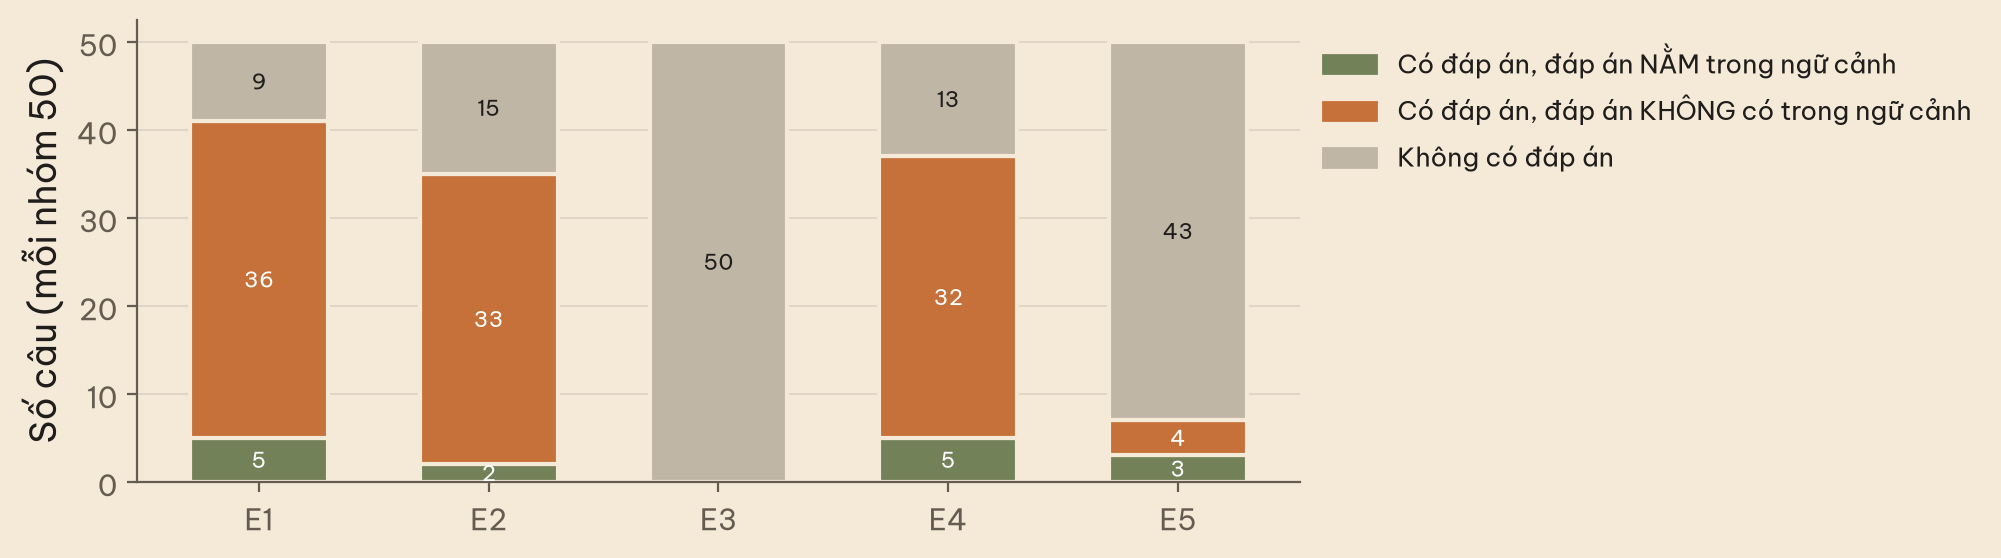
\includegraphics[width=\textwidth]{slide_stress_audit.png}
\end{column}
\begin{column}{0.42\textwidth}
\small
\bignum{\AuditAnsInCtx/\AuditAns}{phobert}\\
câu có đáp án chứa đáp án \emph{trong} ngữ cảnh

\vspace{0.4em}
\footnotesize
$\bullet$ 250 câu dùng chung \AuditCtx{} đoạn văn\\
$\bullet$ E5: 50 câu, \AuditEFiveDistinctQ{} câu hỏi khác nhau\\
$\bullet$ ``Luôn từ chối'' đạt \textbf{\AbstainStressEM} điểm\\[4pt]
\textbf{Nguyên nhân:} \code{\_find\_answer\_start} trả về 0 khi không tìm thấy; ngữ cảnh gán lại theo vòng.

\vspace{0.3em}
\alert{$\Rightarrow$ Không dùng để xếp hạng mô hình.}
\end{column}
\end{columns}
\src{results/stress\_test\_audit.json}
\end{frame}

\begin{frame}{Trần EM do biên từ --- đo được mà không cần mô hình}
\begin{columns}[T]
\begin{column}{0.4\textwidth}
\small
Trên \SegN{} câu có đáp án của validation:

\vspace{0.4em}
\bignum{\SegMisPct\%}{phobert}\\
đáp án cắt ngang một từ (\SegMis{} câu)

\vspace{0.4em}
\bignum{\SegOracle\%}{xlmr}\\
EM tối đa của PhoBERT \emph{hoàn hảo}
\end{column}
\begin{column}{0.56\textwidth}
\footnotesize
\textbf{Đọc từng câu lệch biên:}\\[3pt]
\renewcommand{\arraystretch}{1.25}
\begin{tabular}{@{}l r@{}}
\toprule
\code{pyvi} dính dấu chấm: \code{CNN.} & \MisPeriod \\
\code{pyvi} nối nhầm: \code{Mỹ\_Chú chuột} & \MisMerge \\
Lỗi gán nhãn: ``o thời gian'' & \MisAnnot \\
\textbf{Ranh giới từ ghép thật}: \code{bởi\_vì} & \textbf{\MisCompound} \\
\bottomrule
\end{tabular}

\vspace{0.5em}
\alert{Kênh ``không trả lời được nửa từ'' lấy đi tối đa \SegCeilingLoss{} điểm EM.}
\end{column}
\end{columns}
\src{results/segmentation\_validation.json, results/misaligned\_labels.json}
\end{frame}

% ─────────────────────────────────────────────────────────────── 4 KẾT QUẢ
\section{Kết quả}

\begin{frame}{Kết quả tổng ở ngưỡng mặc định $\tau = 0$ --- validation, \NVal{} câu}
\begin{columns}[T]
\begin{column}{0.58\textwidth}
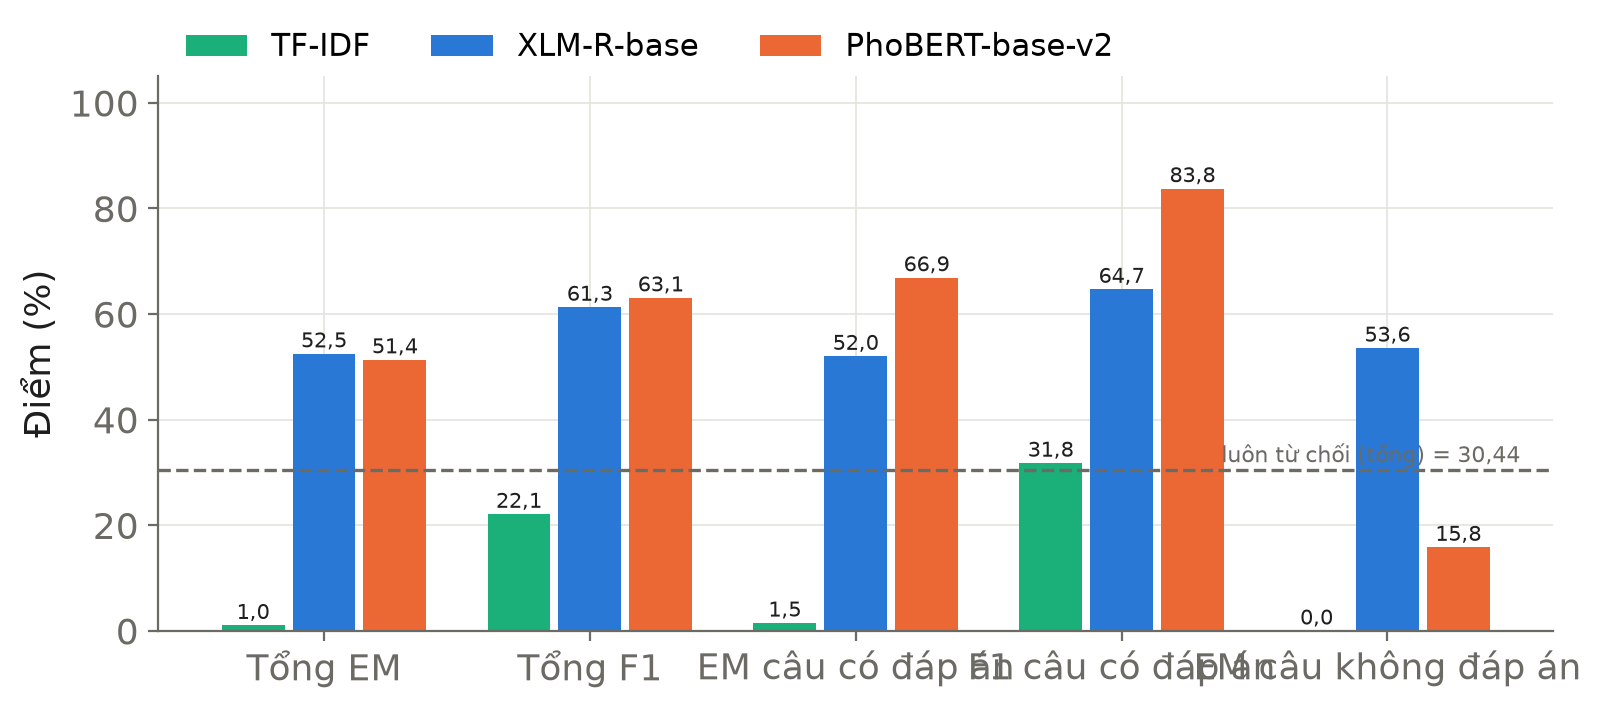
\includegraphics[width=\textwidth]{slide_main_results.png}
\end{column}
\begin{column}{0.4\textwidth}
\small
\begin{tabular}{@{}l r r@{}}
\toprule
& \textbf{EM} & \textbf{F1} \\
\midrule
Luôn từ chối & \AbstainEM & \AbstainFone \\
TF-IDF & \TfidfEM & \TfidfFone \\
\textcolor{xlmr}{\textbf{XLM-R}} s42 & \XlmrEM & \XlmrFone \\
\textcolor{xlmr}{\textbf{XLM-R}} s13 & \XlmrThirteenEM & \XlmrThirteenFone \\
\textcolor{phobert}{\textbf{PhoBERT}} s42 & \PhobertEM & \PhobertFone \\
\textcolor{phobert}{\textbf{PhoBERT}} s13 & \PhobertThirteenEM & \PhobertThirteenFone \\
\bottomrule
\end{tabular}

\vspace{0.6em}
\scriptsize PhoBERT $-$ XLM-R (EM, cùng seed):\\ s42 \textbf{\PairDiff} · s13 \textbf{+\PairSDiff}\\[2pt]
\alert{Hai seed, hai câu trả lời khác nhau!}
\end{column}
\end{columns}
\src{results/eval\_*\_validation.json, results/diagnosis\_validation.json}
\end{frame}

\begin{frame}{Seed 42, $\tau = 0$: hai hồ sơ kỹ năng \emph{ngược nhau}?}
\begin{columns}[T]
\begin{column}{0.48\textwidth}
\centering
\textbf{Câu có đáp án} ({\NValAns})\\[4pt]
\bignum{+\PairAnsDiff}{phobert}\\
\small EM cho PhoBERT\\
\footnotesize CI [\PairAnsLo; \PairAnsHi] · \textcolor{phobert}{\PhobertAnsEM} vs \textcolor{xlmr}{\XlmrAnsEM}
\end{column}
\begin{column}{0.48\textwidth}
\centering
\textbf{Câu không có đáp án} ({\NValImp})\\[4pt]
\bignum{\PairImpDiff}{xlmr}\\
\small EM (PhoBERT kém hơn)\\
\footnotesize CI [\PairImpLo; \PairImpHi] · \textcolor{phobert}{\PhobertImpEM} vs \textcolor{xlmr}{\XlmrImpEM}
\end{column}
\end{columns}

\vspace{1.2em}
\begin{block}{Nhưng PhoBERT từ chối \PhobertAbsRate\%, XLM-R từ chối \XlmrAbsRate\%}
\small Hai chênh lệch phần lớn là \emph{một}: ai sẵn lòng trả lời hơn. Seed 13 \emph{không} có hai hồ sơ ngược
nhau --- PhoBERT từ chối \PhobertThirteenAbsRate\% --- nên hình ảnh này là của \emph{một lần chạy}.
\end{block}
\src{results/diagnosis\_validation.json, results/thresholds.json}
\end{frame}

\begin{frame}{So đúng cách: chọn ngưỡng $\tau$ cho từng mô hình trên dev}
\begin{columns}[T]
\begin{column}{0.5\textwidth}
\small $\tau$ chọn trên dev (\NDevFull{} câu tách từ train), áp \textbf{một lần} lên validation\\[4pt]
\footnotesize
\renewcommand{\arraystretch}{1.2}
\begin{tabular}{@{}l r r r@{}}
\toprule
& $\tau$ & \textbf{F1} & \textbf{Từ chối} \\
\midrule
\textcolor{xlmr}{\textbf{XLM-R}} s42 & \ThrXlmrTau & \ThrXlmrFone & \ThrXlmrAbsRate\% \\
\textcolor{xlmr}{\textbf{XLM-R}} s13 & \ThrXlmrThirteenTau & \ThrXlmrThirteenFone & \ThrXlmrThirteenAbsRate\% \\
\textcolor{phobert}{\textbf{PhoBERT}} s42 & \ThrPhobertTau & \ThrPhobertFone & \ThrPhobertAbsRate\% \\
\textcolor{phobert}{\textbf{PhoBERT}} s13 & \ThrPhobertRunDTau & \ThrPhobertRunDFone & \ThrPhobertRunDAbsRate\% \\
\bottomrule
\end{tabular}

\end{column}
\begin{column}{0.46\textwidth}
\centering
\bignum{+\PairTDiff{} / +\PairSTDiff}{phobert}\\
\small EM cho PhoBERT, seed 42 / seed 13\\
\footnotesize CI theo bài [\PairTArtLo; \PairTArtHi] / [\PairSTArtLo; \PairSTArtHi]\\[6pt]
Phần chia theo loại câu \emph{không} ổn định giữa hai seed
\end{column}
\end{columns}

\vspace{0.3em}
\begin{block}{``Hai hồ sơ ngược nhau'' là do một lần chạy lệch hiệu chỉnh}
\footnotesize Ở ngưỡng đúng, PhoBERT tốt hơn về tổng ở \emph{cả hai} seed. Nhưng phần hơn đó là hiệu chỉnh:
xem slide sau.
\end{block}
\src{results/thresholds.json, results/diagnosis\_validation.json}
\end{frame}

\begin{frame}{Vậy PhoBERT có \emph{đọc} tốt hơn? \alert{Không đo được khác biệt.}}
\begin{columns}[T]
\begin{column}{0.52\textwidth}
\small Phải khớp \textbf{cả hai} biến gây nhiễu: cấu hình cửa sổ và lần chạy sụp đổ.\\[4pt]
\footnotesize PhoBERT s13 vs XLM-R \textbf{256/96}, cả hai ổn định, mỗi bên ở $\tau$ của mình:
\vspace{0.4em}
\renewcommand{\arraystretch}{1.25}
\begin{tabular}{@{}l r l@{}}
\toprule
\textbf{Nhóm câu} & \textbf{Chênh EM} & \textbf{CI 95\%} \\
\midrule
Toàn bộ & \textbf{+\PairMDiff} & [\PairMArtLo; \PairMArtHi] \\
Có đáp án & \textbf{\PairMAnsDiff} & [\PairMAnsArtLo; \PairMAnsArtHi] \\
Không có đáp án & \textbf{+\PairMImpDiff} & [\PairMImpArtLo; \PairMImpArtHi] \\
\bottomrule
\end{tabular}
\end{column}
\begin{column}{0.44\textwidth}
\small
$\bullet$ CI chỉ rộng $\pm$2 điểm $\Rightarrow$ \textbf{không khác biệt}, chứ không phải thiếu dữ liệu\\[4pt]
$\bullet$ Toàn bộ phần hơn nằm ở câu \textbf{không có đáp án}\\[4pt]
$\bullet$ Lát cắt ``cả hai cùng trả lời'' \textbf{đổi dấu} theo lần chạy: \BothMGap{} với seed 13,
\,$-$\BothMSGap{}\, với lr $10^{-5}$

\vspace{0.5em}
\alert{Điều PhoBERT làm tốt hơn là biết khi nào \emph{không} trả lời.}
\end{column}
\end{columns}
\src{results/diagnosis\_validation.json (paired\_matched\_windows\_tuned)}
\end{frame}

\begin{frame}{RQ1 --- Word-level có yếu ở ranh giới từ? \alert{Không.}}
\begin{columns}[T]
\begin{column}{0.5\textwidth}
\small
\renewcommand{\arraystretch}{1.25}
\begin{tabular}{@{}l r r@{}}
\toprule
& \textcolor{xlmr}{\textbf{XLM-R}} & \textcolor{phobert}{\textbf{PhoBERT}} \\
\midrule
EM, khớp biên (\SegAligned) & \XlmrAlEM & \textbf{\PhobertAlEM} \\
EM, lệch biên (\SegMis) & \textbf{\XlmrMisEM} & \PhobertMisEM \\
F1, lệch biên & \XlmrMisFone & \textbf{\PhobertMisFone} \\
\midrule
Lỗi biên / lần trả lời & \XlmrBoundaryRate\% & \PhobertBoundaryRate\% \\
\bottomrule
\end{tabular}
\end{column}
\begin{column}{0.46\textwidth}
\small
$\bullet$ Cơ chế \textbf{có thật}: câu lệch biên, PhoBERT F1 cao mà EM thấp\\
\footnotesize\quad vàng ``trận Gonzales'' $\to$ \code{tại\_trận} $\to$ ``tại trận Gonzales''\\[4pt]
\small $\bullet$ Nhưng chỉ \SegMis{} câu, $p$ = \PairMisP, chặn ở \SegCeilingLoss{} điểm EM\\[4pt]
$\bullet$ Khi đã trả lời, tỉ lệ lỗi biên \textbf{như nhau}

\vspace{0.5em}
\alert{Giả thuyết ghi trước sai hướng.}
\end{column}
\end{columns}
\src{results/diagnosis\_validation.json, results/segmentation\_validation.json}
\end{frame}

\begin{frame}{RQ3 --- Nhận ra câu không có đáp án? \alert{Một phần.}}
\begin{columns}[T]
\begin{column}{0.5\textwidth}
\small
\renewcommand{\arraystretch}{1.25}
\begin{tabular}{@{}l r r r@{}}
\toprule
& \textbf{Từ chối} & \textbf{Prec.} & \textbf{Recall} \\
\midrule
Luôn từ chối & \AbstainAbsRate & \AbstainAbsPrec & \AbstainAbsRec \\
\textcolor{xlmr}{\textbf{XLM-R}} & \XlmrAbsRate & \XlmrAbsPrec & \XlmrAbsRec \\
\textcolor{phobert}{\textbf{PhoBERT}} & \PhobertAbsRate & \PhobertAbsPrec & \PhobertAbsRec \\
\bottomrule
\end{tabular}

\vspace{0.4em}\footnotesize Tỉ lệ câu không có đáp án thật: \PctValImp\%
\end{column}
\begin{column}{0.46\textwidth}
\small
$\bullet$ \textcolor{xlmr}{\textbf{XLM-R}}: từ chối đúng \emph{tần suất}, sai \emph{đối tượng} (\XlmrErrFalseAbs{} câu có đáp án bị từ chối)\\[4pt]
$\bullet$ \textcolor{phobert}{\textbf{PhoBERT}}: gần như không từ chối\\[4pt]
$\bullet$ Rơi vào \textbf{bẫy} của người gán nhãn: câu trả lời sai trùng đúng cụm ``plausible'' ---
PhoBERT \PhobertTrapPct\%, XLM-R \XlmrTrapPct\%
\end{column}
\end{columns}
\src{results/diagnosis\_validation.json}
\end{frame}

\begin{frame}{Vì sao PhoBERT không từ chối? Một sự kiện khi huấn luyện}
\begin{columns}[T]
\begin{column}{0.5\textwidth}
\small Huấn luyện tiếp từ epoch 1, \textbf{cùng batch}, chỉ khác lr:\\[3pt]
\scriptsize
\renewcommand{\arraystretch}{1.1}
\begin{tabular}{@{}l r r r r@{}}
\toprule
& \multicolumn{2}{c}{\textbf{lr $2{,}2\cdot10^{-5}$}} & \multicolumn{2}{c}{\textbf{lr $10^{-5}$}} \\
\textbf{Bước} & \textbf{loss} & \textbf{grad} & \textbf{loss} & \textbf{grad} \\
\midrule
\tabinput{../report/generated/tab_probe_resume_slide.tex}
\bottomrule
\end{tabular}\\[2pt]
loss: ``không có đáp án'' (TB khối 100 bước); grad: chuẩn lớn nhất
\end{column}
\begin{column}{0.46\textwidth}
\small
$\bullet$ Dữ liệu hỏng? \textbf{Không}: \ScanPhobertViolations{} vi phạm / \ScanPhobertFeatures{} feature\\[3pt]
$\bullet$ Tính chất của PhoBERT? \textbf{Không}: epoch 1 từ chối \DevEpochOneAbsRate\% (dev)\\[3pt]
$\bullet$ Bất ổn tối ưu hoá: gradient vọt \textbf{\ResumeHighMaxSpike}, loss ``không đ.án'' kẹt ở \ResumeHighClsEnd; lr $10^{-5}$ thì không\\[3pt]
$\bullet$ Khả năng phân biệt \textbf{còn}: điểm \code{[CLS]} chỉ dịch $\approx$ \ThrPhobertTau{} logit\\[3pt]
$\bullet$ \textbf{Phụ thuộc lần chạy}: seed 13, cùng lr $3\cdot10^{-5}$, không sụp đổ
\end{column}
\end{columns}
\src{results/probe\_resume.json, feature\_scan\_phobert.json}
\end{frame}

\begin{frame}{Mọi lần chạy trên dev: $\tau = 0$ và $\tau$ hiệu chỉnh}
\small F1 trên toàn bộ dev (\NDevFull{} câu tách từ train) --- dữ liệu dùng cho mọi lựa chọn.\\[4pt]
\footnotesize
\renewcommand{\arraystretch}{1.2}
\begin{tabular}{@{}l l r r r r r@{}}
\toprule
& & \multicolumn{2}{c}{\textbf{$\tau = 0$}} & \multicolumn{3}{c}{\textbf{$\tau$ chọn trên dev}} \\
\textbf{Lần chạy} & & \textbf{F1} & \textbf{Từ chối} & $\tau$ & \textbf{F1} & \textbf{Từ chối} \\
\midrule
\tabinput{../report/generated/tab_dev_runs.tex}
\bottomrule
\end{tabular}

\vspace{0.6em}
\small \alert{Hai lần chạy sụp đổ đều là seed 42.} Sau hiệu chỉnh, hai seed PhoBERT gần như trùng nhau; lr $10^{-5}$ ổn định nhưng còn thiếu epoch. Nhóm báo cáo \textbf{hai seed ngang nhau}.
\src{results/thresholds.json, results/training\_curve\_*.json}
\end{frame}

\begin{frame}{RQ2 độ dài · RQ4 baseline · và bộ stress-test}
\begin{columns}[T]
\begin{column}{0.5\textwidth}
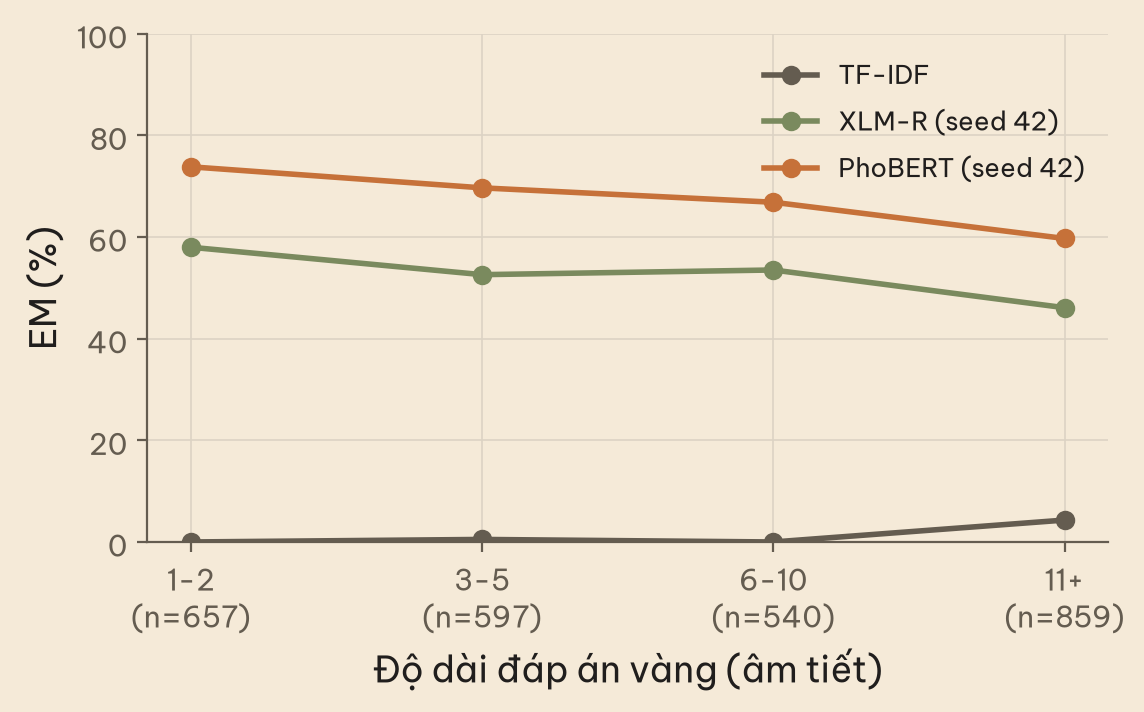
\includegraphics[width=\textwidth]{slide_by_answer_length.png}
\footnotesize \textbf{RQ2:} không suy giảm theo độ dài ngữ cảnh; đáp án dài làm giảm EM (F1 giữ nguyên) như nhau ở cả hai.\\[3pt]
\textbf{RQ4:} Transformer vượt TF-IDF ở mọi nhóm; TF-IDF (EM \TfidfEM) còn thua ``luôn từ chối''.
\end{column}
\begin{column}{0.46\textwidth}
\small \textbf{EM trên stress-test 250 câu}\\[3pt]
\begin{tabular}{@{}l r@{}}
\toprule
\textbf{Luôn từ chối} & \textbf{\AbstainStressEM} \\
XLM-R & \XlmrStressEM \\
PhoBERT & \PhobertStressEM \\
TF-IDF & \TfidfStressEM \\
\bottomrule
\end{tabular}

\vspace{0.5em}
\alert{``Không làm gì'' đứng đầu} --- đúng như kiểm định dự báo. Bộ này không dùng để xếp hạng.
\end{column}
\end{columns}
\end{frame}

% ─────────────────────────────────────────────────────────────── 5 KẾT LUẬN
\section{Kết luận}

\begin{frame}{Kết luận}
\small
\begin{enumerate}
\item \textbf{So ở $\tau$ cố định với một seed là so hiệu chỉnh, không phải năng lực.} Seed 42, $\tau = 0$: ``bằng nhau, hồ sơ ngược nhau''. Ở $\tau$ chọn trên dev: PhoBERT hơn \PairTDiff{} / \PairSTDiff{} điểm EM ở hai seed.
\item \textbf{PhoBERT seed 42 ``không từ chối'' là một sự kiện khi huấn luyện}, tái hiện được, kèm gradient vọt; seed 13 không gặp.
\item \textbf{Không đo được khác biệt về ``đọc''}: khớp cửa sổ thì chênh lệch trên câu có đáp án là \PairMAnsDiff{} điểm. Tách từ cũng không quyết định: chỉ \SegMisPct\% đáp án cắt ngang từ.
\item \textbf{Kiểm định công cụ đo trước khi dùng}: bộ stress-test của chính nhóm xếp ``không làm gì'' đứng đầu.
\end{enumerate}

\vspace{0.4em}
\begin{block}{Giới hạn}
\footnotesize 2 seed · 3 epoch, không tìm siêu tham số · \code{pyvi} thay RDRSegmenter · chưa rõ vì sao sụp đổ ở seed 42 mà không ở seed 13 · validation = public test VLSP (private test ẩn nhãn)
\end{block}
\end{frame}

\begin{frame}{Hướng phát triển}
\small
\begin{itemize}
\item Vì sao sự kiện sụp đổ chỉ xảy ra với PhoBERT; có lặp lại trên CUDA không; warmup dài hơn thay vì hạ lr
\item Huấn luyện thêm epoch (XLM-R và PhoBERT lr $10^{-5}$ còn đang cải thiện); từ 3 seed trở lên
\item PhoBERT với RDRSegmenter; sửa luật dính dấu chấm của \code{pyvi}
\item Xây lại bộ stress-test có kiểm định tự động và câu hỏi do người viết
\end{itemize}

\vspace{1em}
\centering
{\headfont\bfseries\Large Cảm ơn thầy và các bạn đã lắng nghe!}\\[4pt]
\footnotesize Mã nguồn, kết quả và nhật ký: \code{github.com/minhdang900/uit-benchmark-transformer-model-mrc}
\end{frame}

\appendix
\begin{frame}{Phụ lục --- Quá trình huấn luyện}
\begin{columns}[T]
\begin{column}{0.58\textwidth}
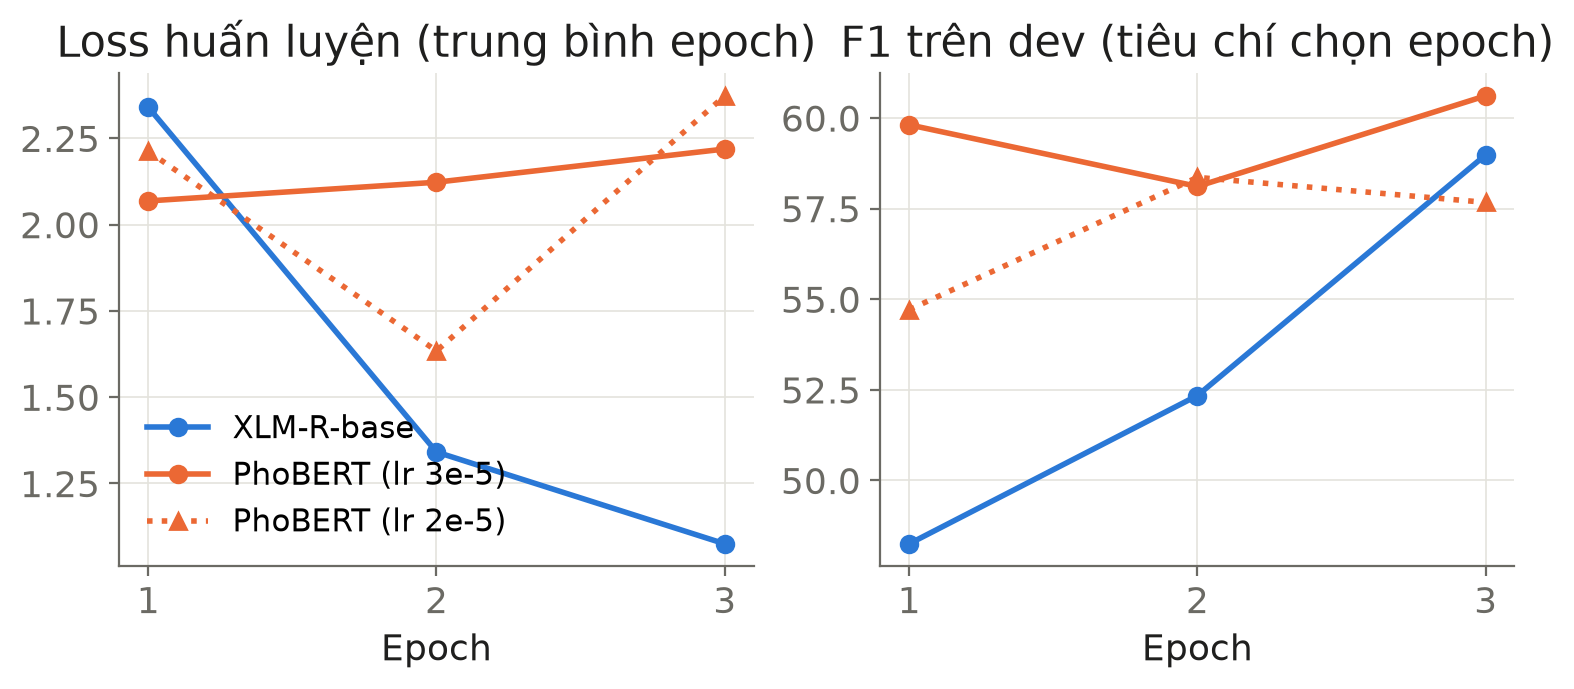
\includegraphics[width=\textwidth]{slide_training_curves.png}
\end{column}
\begin{column}{0.4\textwidth}
\footnotesize
Chọn epoch theo \textbf{F1 trên dev} (tách từ train).\\[3pt]
XLM-R: epoch \XlmrBestEpoch, \XlmrTrainMin{} phút.\\
PhoBERT lr $3\cdot10^{-5}$: epoch \PhobertRunABestEpoch, \PhobertRunATrainMin{} phút.\\
PhoBERT lr $2\cdot10^{-5}$: epoch \PhobertRunBBestEpoch.\\
PhoBERT lr $10^{-5}$: epoch \PhobertRunCBestEpoch.\\
PhoBERT seed 13: epoch \PhobertRunDBestEpoch.\\[3pt]
Hai seed báo cáo ngang nhau.
\end{column}
\end{columns}
\end{frame}

\begin{frame}{Phụ lục --- Độ dao động theo seed và cửa sổ}
\small Validation, EM / F1. Seed tách dev cố định (42) để điểm dev so sánh được.\\[4pt]
\footnotesize
\renewcommand{\arraystretch}{1.2}
\begin{tabular}{@{}l r l r r@{}}
\toprule
\textbf{Mô hình} & \textbf{Seed} & \textbf{Cửa sổ} & \textbf{$\tau = 0$} & \textbf{$\tau$ dev} \\
\midrule
\tabinput{../report/generated/tab_seeds.tex}
\bottomrule
\end{tabular}
\src{results/eval\_*\_validation.json, results/thresholds.json}
\end{frame}



\end{document}
